\documentclass{beamer}
\usepackage{geometry}
\usepackage[english]{babel}
\usepackage[utf8]{inputenc}
\usepackage{amsmath}
\usepackage{amsfonts}
\usepackage{amssymb}
\usepackage{tikz}
\usetikzlibrary{quotes, angles}
\usepackage{graphicx}
\usepackage{multicol}

%\usepackage{pgfplots}
%\pgfplotsset{width=10cm,compat=1.9}
%\usepackage{pgfplotstable}

\setlength{\headheight}{26pt}%doesn't seem to fix warning

\usepackage{fancyhdr}
\pagestyle{fancy}
\fancyhf{}

%\rhead{\small{3 September 2019}}
\lhead{\small{BECA / Dr. Huson / Geometry Unit 1}}

\renewcommand{\headrulewidth}{0pt}

\title{Mathematics Class Slides}
\subtitle{Bronx Early College Academy}
\author{Christopher J. Huson PhD}
\date{7-15 October 2020}

\begin{document}
\frame{\titlepage}
\section[Outline]{}
\frame{\tableofcontents}

\section{1.8 Review vocabulary and segment calculations, 7 October}
  \frame
  {
    \frametitle{GQ: How do we measure line segments?}
    \framesubtitle{CCSS: HSG.CO.A.1 Know precise geometric definitions  \hfill \alert{1.8 Wednesday 7 Oct}}
  
    \begin{block}{Do Now: Self-assessments questions}
    \begin{enumerate}
        \item How do we work efficiently and become a good scholar
        \item What should we know and be able to do
    \end{enumerate}
    \end{block}
    Lesson: Circle definition, trisection \\
    Review and practice of vocabulary, line segments, and congruence
  }

  \frame
  {
    \frametitle{Scholarship assessment}
    \framesubtitle{1: Well below, 2: Approaching, 3: Meets expectations, 4: Exceeds}
  
\includegraphics[width=.95\textwidth]{scholarship-bar-chart.png}
    \begin{enumerate}
      \item Participate: Attendance (Google Classroom), Classkick
      \item Practice assignments: Khan Academy, Deltamath, 1.5 worksheet
      \item Detailed notes: Notebook treasure hunt uploads (weekend)
    \end{enumerate}
  }

  \frame
  {
    \frametitle{What do I know, what can I do assessment}
    \framesubtitle{1: Well below, 2: Approaching, 3: Meets expectations, 4: Exceeds}
  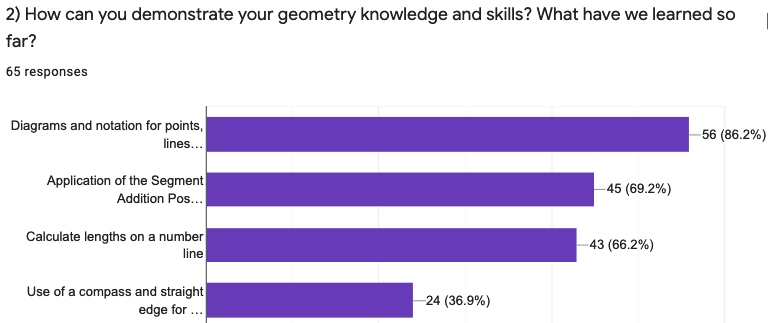
\includegraphics[width=.95\textwidth]{know+do-bar-chart.png}
    \begin{enumerate}
      \item Classkick (open book, timed; use @beca324.org login):\\ Diagrams \& notation, segment addition, number line lengths
      \item Project: Construction of an equilateral triangle
    \end{enumerate}
  }

  \frame
  {
    \frametitle{Definition of a circle in a plane}
      A circle is defined by its center point and radius $r$ as\\
      all the points with distance $r$ to the center. \\[0.5cm]
      Shown below circle $C$, $\rm{radius}=2$\\[0.5cm]
        \begin{tikzpicture}
          \draw [-, thick] (0,0)--(2,0);
          \draw [thick] (0,0) circle [radius=2.0] node[below]{$C$};
          \draw [fill] (0,0) circle [radius=0.05];
          \node at (1,0) [below]{$r = 2$};
        \end{tikzpicture}\\
      Note: All of the radii of a circle are congruent.
  }

  \frame
  {
    \frametitle{Definition: Trisection of a line segment}
      Two points \emph{trisect} a line segment if they divide it into three congruent segments\\[1cm]
      Given $\overline{ABCD}$ with trisecting points $B$ and $C$. If $AD=9$, find ${x}$.\\[1cm]
      \begin{tikzpicture}[scale=0.75]
       \draw [-, thick] (0,0)--(9,0);
       \draw [fill] (0,0) circle [radius=0.05] node[below]{$A$};
       \draw [fill] (3,0) circle [radius=0.05] node[below]{$B$};
       \draw [fill] (6,0) circle [radius=0.05] node[below]{$C$};
       \draw [fill] (9,0) circle [radius=0.05] node[below]{$D$};
       \node at (1.6,0.3) [above]{$x$};
       \node at (4.6,0.3) [above]{$x$};
       \node at (7.6,0.3) [above]{$x$};
       \draw [-, thick] (1.4,-0.2)--(1.4,0.2);
       \draw [-, thick] (1.55,-0.2)--(1.55,0.2);
       \draw [-, thick] (4.4,-0.2)--(4.4,0.2);
       \draw [-, thick] (4.55,-0.2)--(4.55,0.2);
       \draw [-, thick] (7.4,-0.2)--(7.4,0.2);
       \draw [-, thick] (7.55,-0.2)--(7.55,0.2);
       \draw [<->, dashed] (0,-1.3)--(9,-1.3);
       \node at (4.5,-1.3) [below]{$9$};
     \end{tikzpicture} \vspace{1cm}
  }


  \frame
  {
    \frametitle{1) Diagrams and notation}
    Given the points $P$ and $Q$, draw $\overleftrightarrow{PQ}$.\\
    \vspace{2cm}
    \begin{center}
      \begin{tikzpicture}
      \draw [fill] (2,-1) circle [radius=0.05] node[below]{$P$};
      \draw [fill] (5,0) circle [radius=0.05] node[below]{$Q$};
    \end{tikzpicture}
    \end{center} \vspace{1cm}
  }


  \frame
  {
    \frametitle{2) Diagrams and notation}
    Write your answers using proper notation
    \begin{enumerate} 
      \item What is the name of the ray shown in plane $p$
      \item Mark the intersection of $\overrightarrow{JK}$ and $\overleftrightarrow{LM}$ on the diagram and label it $N$.
      \end{enumerate} \vspace{1cm}
      \begin{center}
        \begin{tikzpicture}
        \draw [thick](0,0)--(6,0)--(8,4) node[below left]{$p \ $} --(2,4)--(0,0);
        \draw [->, thick] (2, 1.4)--(6,3);
        \draw [fill] (2.5, 3) circle [radius=0.05] node[below]{$L$};
        \draw [fill] (2, 1.4) circle [radius=0.05] node[below]{$J$};
        %\draw [fill] (3.5,2) circle [radius=0.05] node[below]{$C \ $};
        \draw [fill] (5,2.6) circle [radius=0.05] node[below]{$K$};
        \draw [<->, thick] (2,3.5)--(5.25,.25);
        \draw [fill] (5,0.5) circle [radius=0.05] node[above right]{$M \ $};
      \end{tikzpicture}
    \end{center}
  }

  \frame
  {
    \frametitle{3) Diagrams and notation}
    Sketch a circle centered at point $A$ with radius $AB$.
    \vspace{3cm}
    \begin{center}
      \begin{tikzpicture}
        \draw [thick] (2,0) -- (5,0);
      \draw [fill] (2,0) circle [radius=0.05] node[left]{$A$};
      \draw [fill] (5,0) circle [radius=0.05] node[right]{$B$};
    \end{tikzpicture}
    \end{center} \vspace{3cm}
  }

  \frame
  {
    \frametitle{4)  Diagrams and notation}
      Given isosceles $\triangle XYZ$ with $\overline{XY} \cong \overline{XZ}$.\\[0.5cm]
      On the diagram mark the congruent line segments with tick marks. \vspace{1cm}
      \begin{center}
      \begin{tikzpicture}[scale=0.3]
        \draw [thick](0,0)--(9,0)--(4,8)--(0,0);
        \draw [fill] (0,0) circle [radius=0.05] node[below]{$X$};
        \draw [fill] (9,0) circle [radius=0.05] node[below]{$Y$};
        \draw [fill] (4,8) circle [radius=0.05] node[above right]{$Z$};
      \end{tikzpicture}
      \end{center}
  }

  \frame
  {
    \frametitle{5)  Applying the segment addition postulate}
      Given $\overline{TUV}$, $TU=4.7$, and $UV=6.2$. Find ${TV}$.\\[0.5cm]
      Show your work by marking the diagram and writing an equation.\\[2cm]
        \begin{tikzpicture}
          \draw [-, thick] (0,0)--(7,0);
          \draw [fill] (0,0) circle [radius=0.05] node[below]{$T$};
          \draw [fill] (3,0) circle [radius=0.05] node[below]{$U$};
          \draw [fill] (7,0) circle [radius=0.05] node[below]{$V$};
        \end{tikzpicture} \vspace{4cm}
  }

  \frame
  {
    \frametitle{6) Applying the segment addition postulate}
      Find the perimeter of the isosceles $\triangle ABC$, given $\overline{AC} \cong \overline{BC}$, $AB=7$, and $AC=10$\\[0.5cm]
      Show your work with an equation for full credit.\\
        \begin{tikzpicture}[scale=0.5]
          \draw [thick](0,0)--(4,0)--(2,6)--(0,0);
          \draw [fill] (0,0) circle [radius=0.05] node[below]{$A$};
          \draw [fill] (4,0) circle [radius=0.05] node[below]{$B$};
          \draw [fill] (2,6) circle [radius=0.05] node[above right]{$C$};
          \draw [thick] (0.8,3)--(1.2,3); %tick mark
          \draw [thick] (2.8,3)--(3.2,3); %tick mark
          \node at (2,0) [below]{7};
          \node at (1,3.2) [left]{10};
        \end{tikzpicture}
  }

  \frame
  {
    \frametitle{7) Applying the segment addition postulate}
    Given $\overline{LMN}$, $LM=2x+2$, $MN=15$, $LN=23$. Find ${x}$.
    \begin{center}
       \begin{tikzpicture}
        \draw [-, thick] (0,0)--(7,0);
        \draw [fill] (0,0) circle [radius=0.05] node[below]{$L$};
        \draw [fill] (2,0) circle [radius=0.05] node[below]{$M$};
        \draw [fill] (7,0) circle [radius=0.05] node[below]{$N$};
        \node at (1,0) [above]{$2x+2$};
        \node at (4.5,0) [above]{$15$};
        \draw [<->, dashed] (0,-0.7)--(7,-0.7);
        \node at (3.5,-0.7) [below]{$23$};
      \end{tikzpicture}
    \end{center}
  \begin{enumerate}
      \item Write down an equation to represent the situation. \vspace{0.5cm}
      \item Solve for $x$. \vspace{2cm}
      \item Check your answer. \vspace{2cm}
    \end{enumerate}
  }

  \frame
  {
    \frametitle{8) Applying the segment addition postulate}
      Given equilateral $\triangle ABC$ having perimeter of 21. Find the length of side $\overline{AB}$, $x$. \vspace{1cm}
      \begin{center}
      \begin{tikzpicture}[scale=0.3]
        \draw [thick](0,0)--(9,0)--(4,8)--(0,0);
        \draw [fill] (0,0) circle [radius=0.05] node[below]{$A$};
        \draw [fill] (9,0) circle [radius=0.05] node[below]{$B$};
        \draw [fill] (4,8) circle [radius=0.05] node[above right]{$C$};
        \node at (4.5,0) [below]{$x$};
      \end{tikzpicture}
      \end{center}
  }

  \frame
  {
    \frametitle{9) Finding lengths on the number line}
    Given $E(-3)$ and $F(1)$, as shown on the number line. \\[0.25cm]
    Find the length of the line segment $\overline{EF}$.\\
      \begin{tikzpicture}
        \draw [<->] (-4.5,0)--(4.5,0);
        \draw [-, thick] (-3,0)--(1,0);
        \foreach \x in {-4,...,4} %2 leading for diff!=1
          \draw[shift={(\x,0)},color=black] (0pt,-3pt) -- (0pt,3pt) node[below=5pt]  {$\x$};
          \draw [fill] (-3,0) circle [radius=0.05] node[above] {$E$};
          \draw [fill] (1,0) circle [radius=0.05] node[above] {$F$};
      \end{tikzpicture} \\
      State an equation and the solution. \\[0.5cm]
  Check your work by counting the distance. Leave marks to show your work. \vspace{4cm}  
  }

  \frame
  {
    \frametitle{10) Finding lengths on the number line (spicy)}
    Given $S(1)$ and $T(4)$, as shown on the number line. \\[0.25cm]
    Find point $U$ given that point $T$ bisects $\overline{SU}$. Plot and label $U$ on the number line.\\[0.5cm]
      \begin{tikzpicture}
        \draw [<->] (-1.5,0)--(7.5,0);
        \draw [-, thick] (1,0)--(4,0);
        \foreach \x in {-1,...,7} %2 leading for diff!=1
          \draw[shift={(\x,0)},color=black] (0pt,-3pt) -- (0pt,3pt) node[below=5pt]  {$\x$};
          \draw [fill] (1,0) circle [radius=0.05] node[above] {$S$};
          \draw [fill] (4,0) circle [radius=0.05] node[above] {$T$};
      \end{tikzpicture} \vspace{4cm}  
  }

  \frame
  {
    \frametitle{11) Applying the segment addition postulate}
    Given $M$ is the midpoint of $\overline{AB}$, $AM=3x+6$, $MB=15$.
    \begin{enumerate}
      \item Mark the diagram with the values and tick marks
      \item Write an equation and solve for $x$
      \item Check your result
    \end{enumerate} \vspace{1cm}
      \begin{center}
        \begin{tikzpicture}
          \draw [fill] (0,0) circle [radius=0.05] node[below]{$A$};
          \draw [-, thick] (0,0)--(7,0);
          \draw [fill] (3.5,0) circle [radius=0.05] node[below]{$M$};
          \draw [fill] (7,0) circle [radius=0.05] node[below]{$B$};
          %\node at (1.7,0.5) [above]{$x+2$};
          %\node at (5.2,0.5) [above]{$11$};
          %\draw [<->, dashed] (0,-1)--(7,-1);
          %\node at (3.5,-1) [below]{$20$};
        \end{tikzpicture}
      \end{center} \vspace{4cm}
  }

  \frame
  {
    \frametitle{12) Applying the segment addition postulate}
      The points $Q$ and $R$ trisect the line segment $\overline{PS}$. $PS=13 \frac{1}{2}$.
      \begin{enumerate}
        \item Mark and label the approximate locations of $Q$ and $R$.
        \item Find ${PQ}$. State an equation for full credit.
      \end{enumerate} \vspace{1cm} 
      \begin{center}
        \begin{tikzpicture}
          \draw [-, thick] (0,0)--(7,0);
          \draw [fill] (0,0) circle [radius=0.05] node[below]{$P$};
          \draw [fill] (7,0) circle [radius=0.05] node[below]{$S$};
        \end{tikzpicture} 
      \end{center} \vspace{3cm} 
  }

\end{document}